\documentclass{article}

% if you need to pass options to natbib, use, e.g.:
%     \PassOptionsToPackage{numbers, compress}{natbib}
% before loading neurips_2026

% The authors should use one of these tracks.
% Before accepting by the NeurIPS conference, select one of the options below.
% 0. "default" for submission
\usepackage{neurips_2026}
% the "default" option is equal to the "main" option, which is used for the Main Track with double-blind reviewing.
% 1. "main" option is used for the Main Track
%  \usepackage[main]{neurips_2026}
% 2. "position" option is used for the Position Paper Track
%  \usepackage[position]{neurips_2026}
% 3. "eandd" option is used for the Evaluations & Datasets Track
 % \usepackage[eandd]{neurips_2026}
 % if you want to opt-in for a de-anomymized submission (not recommended, but OK):
 %\usepackage[eandd, nonanonymous]{neurips_2026}
% 4. "creativeai" option is used for the Creative AI Track
%  \usepackage[creativeai]{neurips_2026}
% 5. "sglblindworkshop" option is used for the Workshop with single-blind reviewing
 % \usepackage[sglblindworkshop]{neurips_2026}
% 6. "dblblindworkshop" option is used for the Workshop with double-blind reviewing
%  \usepackage[dblblindworkshop]{neurips_2026}

% After being accepted, the authors should add "final" behind the track to compile a camera-ready version.
% 1. Main Track
 % \usepackage[main, final]{neurips_2026}
% 2. Position Paper Track
%  \usepackage[position, final]{neurips_2026}
% 3. Evaluations & Datasets Track
 % \usepackage[eandd, final]{neurips_2026}
% 4. Creative AI Track
%  \usepackage[creativeai, final]{neurips_2026}
% 5. Workshop with single-blind reviewing
%  \usepackage[sglblindworkshop, final]{neurips_2026}
% 6. Workshop with double-blind reviewing
%  \usepackage[dblblindworkshop, final]{neurips_2026}
% Note. For the workshop paper template, both \title{} and \workshoptitle{} are required, with the former indicating the paper title shown in the title and the latter indicating the workshop title displayed in the footnote.
% For workshops (5., 6.), the authors should add the name of the workshop, "\workshoptitle" command is used to set the workshop title.
% \workshoptitle{WORKSHOP TITLE}

% "preprint" option is used for arXiv or other preprint submissions
 % \usepackage[preprint]{neurips_2026}

% to avoid loading the natbib package, add option nonatbib:
%    \usepackage[nonatbib]{neurips_2026}

\usepackage[utf8]{inputenc} % allow utf-8 input
\usepackage[T1]{fontenc}    % use 8-bit T1 fonts
\usepackage{hyperref}       % hyperlinks
\usepackage{url}            % simple URL typesetting
\usepackage{booktabs}       % professional-quality tables
\usepackage{amsfonts}       % blackboard math symbols
\usepackage{nicefrac}       % compact symbols for 1/2, etc.
\usepackage{microtype}      % microtypography
\usepackage{xcolor}         % colors
\usepackage{graphicx}
\usepackage{amsmath}
\usepackage{amssymb}
\usepackage{multirow}
\usepackage{booktabs}
\usepackage{subcaption}
\usepackage{tcolorbox}
\newcommand{\todo}[1]{\textcolor{red}{TODO: #1}}
\newcommand{\el}[1]{\textcolor{purple}{EL: #1}}
\newcommand{\jk}[1]{\textcolor{blue}{JK: #1}}

% Note. For the workshop paper template, both \title{} and \workshoptitle{} are required, with the former indicating the paper title shown in the title and the latter indicating the workshop title displayed in the footnote. 
\title{Dissecting Reinforcement Learning: Mechanisms Behind Compositional Reasoning in LLMs}


% The \author macro works with any number of authors. There are two commands
% used to separate the names and addresses of multiple authors: \And and \AND.
%
% Using \And between authors leaves it to LaTeX to determine where to break the
% lines. Using \AND forces a line break at that point. So, if LaTeX puts 3 of 4
% authors names on the first line, and the last on the second line, try using
% \AND instead of \And before the third author name.


\author{%
  David S.~Hippocampus\thanks{Use footnote for providing further information
    about author (webpage, alternative address)---\emph{not} for acknowledging
    funding agencies.} \\
  Department of Computer Science\\
  Cranberry-Lemon University\\
  Pittsburgh, PA 15213 \\
  \texttt{hippo@cs.cranberry-lemon.edu} \\
  % examples of more authors
  % \And
  % Coauthor \\
  % Affiliation \\
  % Address \\
  % \texttt{email} \\
  % \AND
  % Coauthor \\
  % Affiliation \\
  % Address \\
  % \texttt{email} \\
  % \And
  % Coauthor \\
  % Affiliation \\
  % Address \\
  % \texttt{email} \\
  % \And
  % Coauthor \\
  % Affiliation \\
  % Address \\
  % \texttt{email} \\
}


\begin{document}


\maketitle


\begin{abstract}
Recently, Large Reasoning Models (LRMs) have achieved impressive performance on reasoning tasks such as mathematics and code generation. LRMs are typically post-trained using supervised fine-tuning (SFT), reinforcement learning (RL), or both, but the mechanisms by which RL leads to reasoning ability remain poorly understood. In this paper, we study RL training mechanisms through the lens of compositional generalization: combining atomic skills to solve more complex problems.
We propose a unified two-axis framework organizing SFT and RL methods along a \emph{data} axis (off-policy to on-policy) and a \emph{loss function} axis (positive-only to positive-plus-negative to GRPO), enabling controlled ablations of individual components. We instantiate this framework on a string-function composition task of increasing depth as well as on competition math.
% \el{as well as on a math domain}.
Our experiments reveal a clear hierarchy among RL components. 
% On-policy data alone is insufficient as positive-only on-policy SFT underperforms teacher-distilled off-policy SFT at higher composition levels. Introducing negative gradients recovers a large fraction of the gap to GRPO, identifying negative samples as the primary driver of compositional ability. Adding a group-mean baseline closes nearly all remaining gap, while full GRPO's standard-deviation normalization contributes relatively little to copositional capability.
% \el{I think it contributes little to this but does to stability, we might want to say "contributes little to compositional capability" etc}.
These findings suggest that GRPO's advantage stems primarily from the joint use of on-policy rollouts and baseline-stabilized negative gradients. More broadly, practitioners can mix and match individual training components to obtain most of RL's benefits, rather than treating RL as a monolithic improvement over SFT.
\end{abstract}



\section{Introduction}
% Hook
Recent advances in Large Language Model (LLM) post-training have produced a new class of systems capable of solving problems that once seemed far beyond reach: competition mathematics, graduate-level science questions, and complex multi-step code generation. The defining ingredient is reinforcement learning with verifiable rewards (RLVR), exemplified by DeepSeek-R1 \citep{deepseek-aiDeepSeekR1IncentivizingReasoning2025} and a wave of follow-up work \citep{deepscaler2025, zengSimpleRLZooInvestigatingTaming2025}
% \el{list a few here}. 
In these systems, a language model generates candidate solutions, a lightweight verifier checks correctness, and the model is updated to produce better solutions over time without human labels. As a result, the resulting models, Large Reasoning Models (LRMs), can produce multi-chain reasoning traces that allow them to solve increasingly complex problems.

% Need and Gap
Yet the mechanisms behind how RL leads to reasoning ability remain poorly understood. At least three explanations compete in the literature. The \emph{discovery} view explains that RL allows the model to discover novel solutions by exploring the solution space and being rewarded accordingly \citep{wenReinforcementLearningVerifiable2025}. On the other hand, the \emph{sharpening} view holds that RL mostly concentrates probability mass on outputs already existing in the base model, improving single-sample accuracy without fundamentally expanding the model's capabilities \citep{yueDoesReinforcementLearning2025}. Finally, the \emph{chaining} view argues that RL implicitly teaches the model to chain multiple skills together, which is necessary to solve complex reasoning problems \citep{setlurE3LearningExplore2025}. Furthermore, it is unclear which components of RL are responsible for the success of RL algorithms like GRPO over standard SFT. Some works argue that the key is the alignment between training data and the model's current distribution \citep{chenRetainingDoingRole2025,mingOneTokenRolloutGuiding2026} while
other works show that RL's use of negative gradients helps the model avoid failure modes \citep{tian_learning_2026} and create reasoning chains \citep{setlurE3LearningExplore2025}. In practice, modern RL pipelines bundle all of these effects together with additional ingredients (KL regularization, variance normalization, entropy shaping), making it difficult to attribute gains to any single cause. 

% Method
This paper addresses this gap by presenting a \textbf{unified framework} that decomposes training into two orthogonal axes. The first axis is \textbf{data}: we compare teacher-generated off-policy data, base-model bootstrapped data, and fully on-policy rollouts, asking how the source of training trajectories affects compositional performance. The second axis is the \textbf{loss function}: starting from the SFT loss function (positive samples only), we progressively introduce negative gradient updates, a group mean baseline, and variance normalization, arriving at the full GRPO objective. By crossing these two axes we construct a grid of training methods that interpolates between standard off-policy SFT and standard GRPO, isolating the contribution of each component and creating a \emph{unified framework} to understand existing post-training paradigms. 
We investigate training mechanisms through the lens of \emph{compositional generalization}: the ability to chain multiple known atomic skills together to solve more complex problems. As sample tasks, we use string functions \citep{yuanLLMsLearnNewSkills2025} and competition math \citep{deepscaler2025}.
% \el{This paragraph is very repetitive, you may want to merge it with the previous one}

% Task
% We investigate training mechanisms through the lens of \emph{compositional generalization}: the ability to chain multiple known atomic skills together to solve more complex problems. 
% Crucially, the gap between SFT and RL is especially pronounced here: SFT-trained models plateau sharply as composition depth increases, while RL-trained models continue to improve, creating a clean and measurable performance separation \citep{yuanLLMsLearnNewSkills2025, cheng_atomic_2025}.
% This is important, as compositional generalization is a key ingredient in general reasoning ability \citep{yueDoesReinforcementLearning2025, park_how_2025}. A model solving a complex problem may need to decompose the task into multiple sub-tasks and solve each sub-task sequentially. 
% We use the string-function composition task introduced by \citet{yuanLLMsLearnNewSkills2025}, where the model must predict the output of composed string transformations of increasing depth.
% \el{Also explain math task}


% Results/Findings
\todo{summarize results and organize findings/contributions}


\el{Overall I think this intro is a little long-winded/repetitive, I think it can probably be condensed to three or four paragraphs: past work/theories, what we do, findings, and then contributions}



\section{The Task: Compositional Generality}

\todo{framing: generalization across composition vs difficulty}

\subsection{Task Definition}
Compositional generalization is the ability to compose multiple atomic skills to solve a harder problem. Hence, benchmarks for compositional ability define the notion of an atomic skill and construct more complex tasks by composing these skills. Generally, we can measure the difficulty of the task by the amount of composition required to solve it. To make this more concrete, we study a toy task where the goal is to predict the output of functions that map strings to strings \citep{yuanLLMsLearnNewSkills2025}. Compositional generalization is important for a model to generalize to new tasks, especially in domains like coding and math. There may be relatively few procedures to learn, but the key point of difficulty is applying learned operations in the correct situations and alongside other techniques.

\subsection{Toy Task: String Functions}
\label{sec:string-function}
Our first experiments are on the string-function setting as proposed in \citet{yuanLLMsLearnNewSkills2025}. The model receives definitions of simple atomic functions and must predict outputs of composed programs.
Note that difficulty is controlled by composition depth. A level-$i$ task requires composing $i$ operations. Figure \ref{fig:string-function} shows an example of string functions in this dataset. The dataset contains 25 unique string functions, split into 13 in the train set and 12 in the eval set. Note that with $i$ composed functions, any combination of string functions is a valid task, leading to exponentially many tasks as a function of $i$.

\begin{figure}[h!]
\centering
\includegraphics[width=\textwidth]{imgs/string-function.png}
\caption{Overview of the string function task \el{May want to make a single figure showing both domains and put more detail about the setting in case people don't read the setup}}
\label{fig:string-function} 
\end{figure}


We follow the training protocol proposed in \citet{yuanLLMsLearnNewSkills2025}. For any pretrained model, we \emph{initialize} the model by training it on level-1 tasks with standard Supervised Fine-Tuning (SFT). This ensures that the model masters the atomic tasks. We call the resulting checkpoint \textbf{Base}, which is used as the starting point for compositional training.
\begin{itemize} 
\item \textbf{Compositional Training:} To train for composition, we train on level-2 tasks starting from \textbf{Base}. We use level-2 tasks since they are the lowest difficulty tasks that requires composition. We train using various post-training methods including SFT, DPO, and GRPO, and analyzing their effectiveness.
\item \textbf{Evaluation:} We measure performance on a separate evaluation set on tasks from level 1 to level 8. This allows us to see how performance extrapolates to higher composition levels.
\end{itemize}

% \el{I feel this isn't really clear, so all models undergo both stage 1 and 2 training and then are evaluated on higher levels right? and we only vary stage 2 posttraining, and not stage 1? can maybe be a bit more explicit about this}
% \jk{yes that is correct. Updated above to make this more clear, but lmk}

\subsection{Real life Task: Math}
We further study post-training algorithms with a more realistic task: mathematics. We use the training dataset from DeepScaleR \citep{deepscaler2025}, a collection of competition math problems. Following \citet{setlurE3LearningExplore2025}, we split dataset into easy, medium, and hard based on accuracy of a larger QwQ-32B model. The easy set contains problems with accuracy greater than 70\%, the hard set contains problems with accuracy less than 15\%, and the medium set contains problems in between. We train on the easy and medium set and evaluate on all three difficulties to see how the model generalizes to harder difficulty problems.




\section{Method: Decomposing Training Mechanisms}
% 3  Decomposing Training Mechanisms
%    3.1  A Unified Two-Axis Framework  [short intro establishing the grid]
%    3.2  Data Axis: Off-Policy to On-Policy
%         - Source (Teacher / Bootstrap / Iterative / On-policy)
%         - Note on filtering as a secondary degree of freedom
%    3.3  Loss Function Axis: Positive-Only to GRPO
%         - Lead with the weighting table
%         - Derive SFT → POS+NEG → REINFORCE+ → GRPO as special cases
%         - GRPOMask as diagnostic ablation
%    3.4  Relationship to DPO  [short, positioned as "outside the linear regime"]

\subsection{A Unified Two-Axis Framework}
\label{sec:methods}

\begin{table}[t]
\centering
\caption{The unified two-axis framework with representative examples.}
\label{tab:unified-framework}

\setlength{\arrayrulewidth}{0.4pt}
\renewcommand{\arraystretch}{1.15}

\begin{tabular}{|l|c|c|}
\hline
& \textbf{Positive samples only}
& \textbf{Positive and negative samples} \\
\hline
\textbf{Off-policy} & SFT & DPO \\
\hline
\textbf{On-policy} & On-policy SFT & GRPO \\
\hline
\end{tabular}
\end{table}

Our goal is to decompose the training mechanisms across various SFT and RL methods and organize them into a unified framework. As a starting point, we identify the two core factors that differentiate SFT with GRPO: on-policy data and use of negative samples for gradient updates. Table \ref{tab:unified-framework} classifies known post-training methods into a two-axis grid, which allows us to place popular post-training algorithms like SFT, DPO, and GRPO.
We generalize the two components into the following axis:
\begin{itemize}
    \item \textbf{Data}: this involves the way we source and select data that will be used for training. 
    \item \textbf{Loss function}: this involves the way we update the model parameters based on the data.
\end{itemize}
   
\subsection{Data Axis}
% A key ingredient in post-training is the data. We first consider the source of the data, then consider how we can curate and filter it. \el{This is a really obvious point, maybe we can just delete this paragraph...}

% \subsubsection{Data Source}
One common distinction between methods in RL is whether the data is on-policy or off-policy. On-policy data is generated by the current model being trained, while off-policy data is generated by a previous reference model, humans, or teacher models. To study the role of data source, we formalize the following settings:

\begin{itemize}
    \item \textbf{Teacher}: teacher-generated trajectories
    \item \textbf{Bootstrap}: bootstrapped trajectories from the initial model checkpoint
    % \item \textbf{Iterative}: bootstrapped trajectories from the previous model checkpoint. We can control the number of model checkpoints, $k$, to use for bootstrapping. If $k=1$, it is the same as Bootstrap-SFT. If $k=\text{number of training steps}$, it is the same as On-policy SFT.
    \item \textbf{On-policy}: on-policy trajectories throughout training
\end{itemize}

\begin{table}[t]
  \centering
  \caption{Classification of data-source methods.}
  \label{tab:data-source-classification}

  \renewcommand{\arraystretch}{1.15}

  \begin{tabular}{|l|l|}
    \specialrule{\heavyrulewidth}{0pt}{0pt}
    \textbf{Data source} & \textbf{Classification} \\
    \hline
    \textbf{Teacher} & Off-policy \\
    \hline
    \textbf{Bootstrap} & Off-policy \\
    \hline
    % \textbf{Iterative ($k$)} & Off-policy \\
    % \hline
    \textbf{On-policy} & On-policy \\
    \specialrule{\heavyrulewidth}{0pt}{0pt}
  \end{tabular}
\end{table}

We consider the \textbf{Teacher} and \textbf{Bootstrap} settings as Off-policy methods since they make gradient updates based on data from older models or teacher models. 
% However, we can still smoothly transition from Off-policy to On-policy methods by increasing the number of model checkpoints used in the \textbf{Iterative} setting.

% \todo{Second ablation method: interesting?}
% Another way to control the data source is to use a mixture of off-policy and on-policy data \citep{yanLearningReasonOffPolicy2025}. At each training step, we generate on-policy samples and mix this with some existing set of off-policy samples. We call this setting \textbf{Mixture($p$)} where we can control $p$, the proportion of on-policy samples.


% \subsubsection{Data Policy}
% Data policy refers to the way we curate data for training. In addition to controlling the data source via on-policy vs off-policy methods mentioned previously, we can also apply additional filtering strategies to the data. For verifiable tasks, it is common practice to filter based on correctness ratios or trajectory lengths.
% For example, when training with GRPO, we can filter out groups that have 100\% accuracy or 0\% accuracy since this will result in a zero update signal.
% A common approach in fine-tuning is to use Rejection Fine-Tuning (RFT), which only trains on correct samples.
% We can use more complex data policy methods such as filtering out groups with accuracy above $\text{threshold}_{\text{high}}$ or below $\text{threshold}_{\text{low}}$. 
% \todo{This is probably not too interesting. Maybe remove this section}


\subsection{Loss Function Axis}
Our key insight is that we can view \emph{loss functions as methods that apply different weights to positive and negative samples.} Table \ref{tab:loss_function_comparison} summarizes how different loss functions weight positive and negative samples. Note that this understanding applies for tasks with binary reward ($r \in \{1, 0\}$).

\begin{table}[h!]
\centering
\begin{tabular}{clcc}
\toprule
\textbf{Use of Negative Samples} & \textbf{Loss Function} & \textbf{Positive Weight} & \textbf{Negative Weight} \\
\midrule
% \multirow{2}{*}{No}
No & SFT (\ref{eq:SFT}) & $1$ & $0$ \\
% & GRPOMask (\ref{eq:GRPOMask}) & $(1 - \mu)/\sigma$ & $0$ \\
\midrule 
\multirow{3}{*}{Yes} & POS+NEG (\ref{eq:POS+NEG}) & $1$ & $-1$ \\
& REINFORCE+ (\ref{eq:REINFORCE+}) & $1 - \mu$ & $- \mu$ \\
& GRPO (\ref{eq:GRPO}) & $(1 - \mu)/\sigma$ & $-\mu/\sigma$ \\
\bottomrule
\end{tabular}
\label{tab:loss_function_comparison}
\vspace{0.5em}
\caption{Comparison of loss functions by weights used for positive and negative samples.}
\end{table}

First, we start with the standard loss function for Supervised Fine-Tuning (SFT).

\[ \ell_{\text{SFT}}(\theta) = - \mathbb{E}_{(x, y)} \left[ \frac{1}{T} \sum_{t = 1}^T \log \pi_\theta(y_t \vert x, y_{< t}) \right] \]

For consistency with RL training procedures, we consider SFT as generating multiple rollouts for the same problem instance and filtering the positive samples for training. Let $G$ denote the number of generated samples per problem. Furthermore, we can rewrite the following term:
\[
    \log \pi_\theta(y \vert x) = \Sigma_{t = 1}^T \log \pi_\theta(y_t \vert x, y_{< t})
\]

Then, the loss simplifies to 
\[
    \ell_{\text{SFT}}(\theta) = - \mathbb{E}_{(x, \{y\}^{G^+})} \left[ \frac{1}{G} \sum_{i = 1}^G \frac{1}{T} \log \pi_\theta(y_i \vert x) \right]
\]
where $G^+$ denotes the set of positive samples.

Since SFT only uses positive samples, we can rewrite the loss as:
\begin{equation}
    \ell_{\text{SFT}}(\theta) = - \mathbb{E}_{(x, \{y\}^G)} \left[ \frac{1}{G} \sum_{i = 1}^G \boldsymbol{1}[r_i = 1] \cdot \frac{1}{T} \log \pi_\theta(y_i \vert x) \right]
    \label{eq:SFT}
    % \tag{SFT}
\end{equation}

This derivation demonstrates that SFT is a special case where positive samples have weight 1 and negative sample have weight 0.

As a simple way to incorporate negative samples, we have the following loss function that increases likelihood of positive samples and decreases likelihood of negative samples:
\begin{equation}
    \ell_{\text{POS+NEG}}(\theta) = - \mathbb{E}_{(x, \{y\}^G)} \left[ \frac{1}{G} \sum_{i = 1}^G \boldsymbol{1}[r_i = 1] \cdot \log \pi_\theta(y_i \vert x) - \boldsymbol{1}[r_i = 0] \cdot \log \pi_\theta(y_i \vert x) \right]
    \label{eq:POS+NEG}
    % \tag{POS+NEG}
\end{equation}

This is essentially equivalent to REINFORCE \citep{williamsSimple1992} with rewards $r_i \in \{1, -1\}$ instead of $\{1, 0\}$. In other words, the loss function simply places $+1$ weight on positive samples and $-1$ weight on negative samples.

Next, we can further add a baseline to the REINFORCE loss where $\mu$ is the mean reward of the group:
\begin{equation}
    \ell_{\text{REINFORCE+}}(\theta) = - \mathbb{E}_{(x, \{y\}^G)} \left[ \frac{1}{G} \sum_{i = 1}^G (r_i - \mu) \cdot \log \pi_\theta(y_i \vert x) \right]
    \label{eq:REINFORCE+}
    % \tag{REINFORCE+}
\end{equation}

This takes into account the relationship of samples within $G$. If most samples in the group are correct, then the mean is high and the weight on each positive sample is low. On the other hand, if only a few samples are correct, the mean is low and the weight on positive samples are high. The same is true for negative samples. Hence, we can see loss \ref{eq:REINFORCE+} as placing $1- \mu$ weight on positive samples and $-\mu$ weight on negative samples.


Finally, we use standard deviation $\sigma$ as a normalization factor to get to GRPO loss.
\begin{equation}
    \ell_{\text{GRPO}}(\theta) = - \mathbb{E}_{(x, \{y\}^G)} \left[ \frac{1}{G} \sum_{i = 1}^G \left( \frac{r_i - \mu}{\sigma} \right) \cdot \log \pi_\theta(y_i \vert x) \right]
    \label{eq:GRPO}
\end{equation}

For simplicity, we do not consider clipping and KL-divergence penalty. In this simplified version, we see that GRPO loss weighs the samples using a group-normalized advantage: $\frac{1- \mu}{\sigma}$ for positive samples and $\frac{-\mu}{\sigma}$ for negative samples.


% Another setting used to isolate the effect of negative gradients is to apply a mask to the negative gradients in GRPO \citep{setlurE3LearningExplore2025}.
% \begin{equation}
%     \ell_{\text{GRPOMask}}(\theta) = - \mathbb{E}_{(x, \{y\}^G)} \left[ \frac{1}{G} \sum_{i = 1}^G \boldsymbol{1}[r_i = 1] \cdot \left( \frac{r_i - \mu}{\sigma} \right) \cdot \log \pi_\theta(y_i \vert x) \right]
%     \label{eq:GRPOMask}
%     % \tag{GRPOMask}
% \end{equation}


% \subsubsection{Relation to DPO}
% \todo{This is sort of just POS+NEG setting with non-linearity + KL divergence. Fit this into framework as secondary axis?}

% DPO is another method that uses negative samples. It is defined as:

% $$ \ell_{\text{DPO}}(\theta) = - \mathbb{E}_{(x, y^+, y^-)} \left[ \log \sigma\left( \beta \left( \log \frac{\pi_\theta(y^+ \mid x)}{\pi_{\text{ref}}(y^+ \mid x)} - \log \frac{\pi_\theta(y^- \mid x)}{\pi_{\text{ref}}(y^- \mid x)} \right) \right) \right]$$
% Intuitively, DPO incentivizes the likelihood of the positive sample to be greater than the likelihood of the negative sample. Since DPO applies a non-linear function to the difference of the log probabilities, it does not fit into the derivation from SFT to GRPO loss above.
% Instead, DPO is an alternative way to introduce negative gradients outside of the main axis we examine.


% \el{We shouldn't say it doesn't fit into the framework since this sounds weird. it does fit in the 2x2 grid but we can mention it as an alternative way to introduce negative gradients outside the main axis we examine}

\el{TODO: add a theory part here about tree structure in rollout}

\section{Experiments}
\label{sec:experiments}
\subsection{Setup}
\subsubsection{Toy task: string functions}
We use Llama-3.1-8B-Instruct as the backbone model. As noted in section \ref{sec:string-function}, we first train this model on level-1 tasks to ensure that the model has acquired the atomic skills. This setup stage uses Rejection Fine-Tuning (RFT) on 117k samples. We call the resulting checkpoint \textbf{Base}, which is used as the starting point for our main training methods.
During \textbf{Compositional Training}, we train the \textbf{Base} model with various training methods as described in section \ref{sec:methods}. By evaluating the performance of the model on level-$i$ tasks with $i \ge 2$, we can measure the compositional generalization ability of the model.

% To conduct a fair comparision between methods, we utilize a matched compute setting, where compute is measured by the number of samples used in the training process. For On-policy methods, let $b$ be the batch size and $T$ be the total training steps. For each problem instance, we rollout $G$ samples (this is also the group size in GRPO). Then, the total number of samples used is $bTG$. For Off-policy methods, we use the teacher model or checkpoint model to generate $G$ solutions for $bT$ problem instances, matching the total sample count. One thing to note is that when we use SFT loss, we only use positive samples. However, we still measure the compute by the total number of samples \emph{before} filtering out the negatives. By default, we use a batch size of $b=16$ and $T=1200$ training steps, resulting in $19200$ unique problem instances. We use group size of $G=16$, resulting in total sample count of $307200$.

\subsubsection{Real Life Task: Math}
Following the setup in \citet{setlurE3LearningExplore2025}, we use Qwen3-1.7B as the base model. 
\el{Was there a justification for using a different base model here?} \jk{following e3 setup} 
We split the dataset into easy, medium, and hard subsets based on accuracy of a larger QwQ-32B model. We train the model on first the easy split followed by medium. Throughout training, we evaluate performance on a held out validation set of easy, medium, and hard. By observing performance on the hard validation set, we can see the generalization performance on harder problems not seen during training. 


% \subsection{Baselines}
% In order to understand the effect of different components, we establish lower and upper bounds for performance. Namely, the standard off-policy bootstrap SFT method establishes the baseline lower bound performance. On the other hand, standard on-policy GRPO establishes our gold-standard upper bound in performance. Figure \ref{fig:baselines} shows the performance gap, which we hope to close by ablating various components.

% \begin{figure}[h!]
% \centering
% \includegraphics[width=0.8\textwidth]{imgs/baseline.png}
% \caption{Accuracy comparing the Base model to 2 training methods: SFT and GRPO}
% \label{fig:baselines}
% \end{figure}

\subsection{Results}
\begin{figure}[h!]
\centering
\includegraphics[width=0.8\textwidth]{imgs/result-table-zones.jpg}
\caption{Classification of trained model behavior into 3 zones 
% \el{is there no difference between teacher and bootstrap? if not we could just remove the partition for simplicity}
}
\label{fig:zones}
\end{figure}

We train the same base model using the training recipe for each combination of data source and loss functions. We observe that the training dynamics can be classified into 3 meaningful zones (Figure \ref{fig:zones}): 
\begin{itemize}
    \item \textbf{Mimic Zone}: This zone contains off-policy SFT methods, which train the model to mimic the distribution of the data and does not generalize well to higher compositions and difficulties.
    \item \textbf{Collapse Zone}: This zone contains combinations of off-policy data with negative gradients. The high gradient norms from off-policy data creates instability during training, resulting in model collapse to degenerate behavior.
    \item \textbf{Generalization Zone}: In the on-policy setting, we show that models can achieve good generalization. However, on-policy SFT method can result in training collapse while the introduction of negative gradients result in reliable training. We show that naively adding negative gradients with POS+NEG setting can recover most of the performance, but GRPO achieves the best results overall.
\end{itemize}


\subsection{Mimic Zone}

When using SFT with off-policy data, the results show meaningful improvement over the base model, but significantly lags behind RL methods like on-policy GRPO (Figure \ref{fig:mimic-accuracy-string}).
As expected, the response length distributions after training (Fgure \ref{fig:sft_response_length}) show that it matches the distribution of the data source.
The distribution in the Bootstrap setting is similar to the \textbf{Base} model since the data used during training comes from the initial model checkpoint. On the other hand, the teacher data comes from the On-policy GRPO checkpoint, which leads the model to imitate the long chain-of-thought trajectories. As a result, Teacher data outperforms Bootstrap data since the longer chain-of-thought examples generalize better to unseen samples.

Table \ref{tab:mimic-zone-numbers} reports the underlying accuracy numbers. At Level 2, Teacher-SFT (36.7\%) clearly outperforms Bootstrap-SFT (24.2\%) and On-policy-SFT (28.5\%), confirming that the quality/length of the off-policy source distribution matters, not just whether data is off-policy versus on-policy; averaged over levels 1--5, Teacher-SFT (25.3\%) still leads Bootstrap-SFT and On-policy-SFT, which land within 0.1pp of each other (21.6\% each). This also answers whether the Teacher/Bootstrap partition in Figure \ref{fig:zones} is meaningful: at low composition depth the two off-policy sources behave very differently (a 12.5pp gap at Level 2), so the partition should be kept.

\begin{table}[h!]
\centering
\begin{tabular}{lcccccc}
\toprule
\textbf{Method} & \textbf{L1} & \textbf{L2} & \textbf{L3} & \textbf{L4} & \textbf{L5} & \textbf{Avg (L1--L5)} \\
\midrule
Base & 74.6\% & 12.5\% & 2.3\% & 0.8\% & 0.4\% & 18.1\% \\
Bootstrap-SFT & 74.2\% & 24.2\% & 5.9\% & 2.7\% & 1.2\% & 21.6\% \\
On-policy-SFT & 69.1\% & 28.5\% & 6.6\% & 2.7\% & 1.2\% & 21.6\% \\
Teacher-SFT & 77.7\% & 36.7\% & 9.0\% & 3.1\% & 0.0\% & 25.3\% \\
\bottomrule
\end{tabular}
\caption{Mimic Zone: accuracy by composition level for the Base model and the three SFT variants (data from \texttt{results/main.csv}, \texttt{results/baseline.csv}).}
\label{tab:mimic-zone-numbers}
\end{table}

\textbf{Key Finding}: SFT loss trains the model to \emph{mimic} the distribution of the data source, but doesn't generalize well.

\begin{figure}[h]
\centering
\begin{subfigure}[b]{0.38\textwidth}
    \centering
    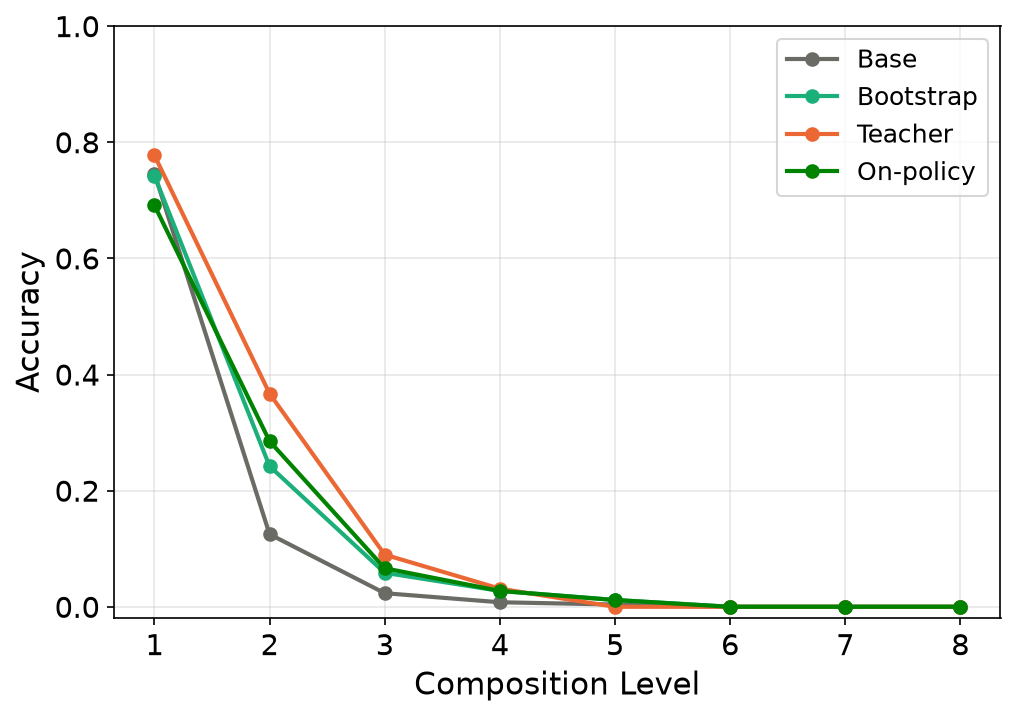
\includegraphics[width=\textwidth]{imgs/data_vary_loss_fn_sft_no_onpolicy.png}
\caption{Accuracy comparing Off-policy and On-policy SFT methods on string function task.}
\label{fig:mimic-accuracy-string}
\end{subfigure}
\hfill
\begin{subfigure}[b]{0.58\textwidth}
    \centering
    % \jk{TODO: this panel needs regenerating. scripts/analysis/plot_response_length_eval.py tokenizes
    % the raw eval rollout .parquet files, which live only on the cluster at
    % /data/user_data/gyeongwk/checkpoints/string-task/*/rollout_eval_data/ -- not reconstructable
    % from wandb history (these SFT runs only logged system/train/val-loss metrics, no response-length
    % keys). Re-run that script against the cluster checkpoints and drop the output at this path.}
    \includegraphics[width=\textwidth]{imgs/sft_eval_response_length_no_onpolicy.png}
\caption{Response length distribution on evaluation set for models trained with SFT on string function task.}
\label{fig:sft_response_length}
\end{subfigure}
\caption{}
\label{fig:mimic-zone}
\end{figure}

The same Mimic Zone pattern holds on the math task. Figure \ref{fig:math-bootstrap-sft} shows Math Bootstrap-SFT (trained only on the easy split, frozen base-model rollouts): easy-set pass@1 rises modestly from 61.7\% to 65.5\% over 550 steps, while medium (10.1\%$\to$10.2\%) and hard (4.5\%$\to$4.4\%) are essentially flat throughout training. Bootstrap-SFT mimics the frozen data distribution well enough to make small in-distribution gains but shows no transfer to harder problems.

\begin{figure}[h!]
\centering
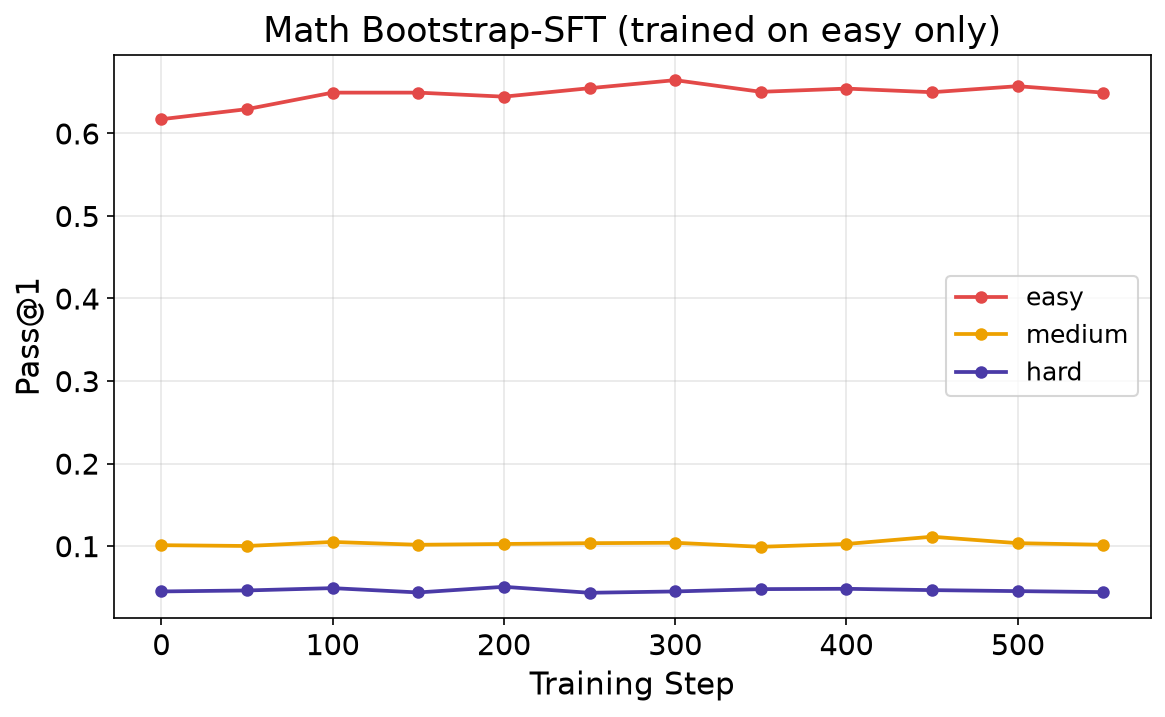
\includegraphics[width=0.6\textwidth]{imgs/math_bootstrap_sft_pass1.png}
\caption{Math Bootstrap-SFT (trained on easy split only): pass@1 on easy/medium/hard validation sets over training.}
\label{fig:math-bootstrap-sft}
\end{figure}

\subsection{Collapse Zone}
When combining off-policy data with negative samples, we observe a collapse in training, leading to a worse model than the base model. Table \ref{tab:collapse-zone-numbers} reports train-pool accuracy at the last available checkpoint for each run: Bootstrap-GRPO collapses fastest and hardest, from 12.2\% at step 100 to 0.4\% by step 661 (99.4\% of responses hit the length cap without emitting an answer), with the optimizer itself blowing up (\texttt{actor/grad\_norm}=18{,}362, \texttt{actor/perplexity}=$\infty$ at the final step). Bootstrap-REINFORCE+Baseline degenerates in output form just as fast (81\% length-capped by step 260) but its accuracy stays around 9.6\% in the window observed. Teacher-GRPO and Teacher-REINFORCE+Baseline, trained on the much higher-quality distilled pool, degrade more gradually but show the same monotonic trend, reaching 8.8\% (step 600) and 4.7\% (step 1033) respectively with no sign of a floor.

\begin{table}[h!]
\centering
\begin{tabular}{lccc}
\toprule
\textbf{Run} & \textbf{Last step} & \textbf{Accuracy} & \textbf{\% length-capped} \\
\midrule
Bootstrap-GRPO & 661 & 0.4\% & 99.4\% \\
Bootstrap-REINFORCE+Baseline & 260 & 9.6\% & 81\% \\
Teacher-GRPO & 600 & 8.8\% & 82\% \\
Teacher-REINFORCE+Baseline & 1033 & 4.7\% & 93\% \\
\bottomrule
\end{tabular}
\caption{Collapse Zone: terminal train-pool accuracy and fraction of generations that hit the length cap without a terminated answer, for off-policy runs with negative-sample losses (from \texttt{reports/string\_task\_offpolicy\_collapse.md}, corroborated by wandb).}
\label{tab:collapse-zone-numbers}
\end{table}

Gradient norms confirm the instability directly: Figure \ref{fig:grad-norm-collapse} plots \texttt{actor/grad\_norm} on a log scale for all four off-policy+negative-gradient runs against the full on-policy band. On-policy training holds a tight $0.1$--$0.5$ range throughout; every off-policy run breaks out of that range within the first 100--200 steps and reaches $10^3$--$10^5$ (peaking above $5\times10^5$ for Bootstrap-GRPO) --- four to five orders of magnitude larger, not just qualitatively "orders of magnitude greater." This leads to training instability, causing models to collapse to degenerate behavior including token-level loops.

\begin{figure}[h!]
\centering
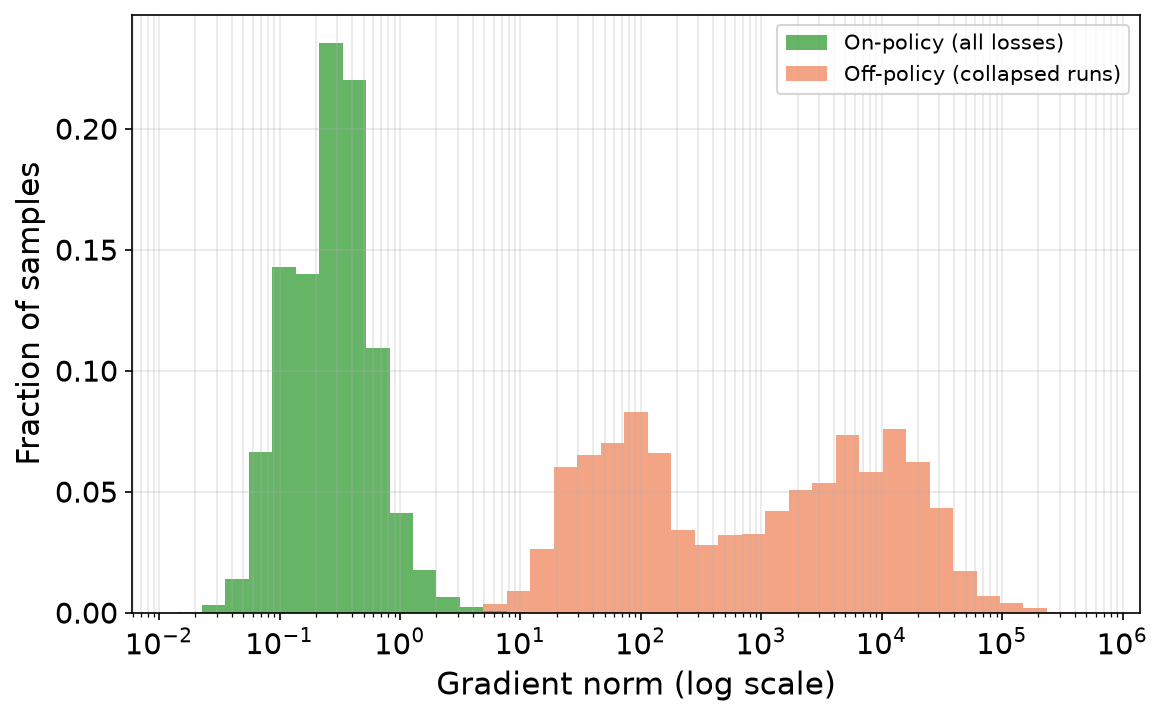
\includegraphics[width=0.7\textwidth]{imgs/grad_norm_collapse.png}
\caption{Gradient norm (log scale) over training: on-policy band (all four loss functions) versus the four off-policy runs that collapse. Off-policy runs run out of steps because the jobs crashed or were killed once collapsed, not because training was scheduled to stop early.}
\label{fig:grad-norm-collapse}
\end{figure}

\begin{tcolorbox}[colback=gray!5, colframe=gray!40, title=Example Generation 1 (Bootstrap GRPO), fonttitle=\bfseries]
To predict the output of `main\_solution("kqqqqqq...(repeats q token until token limit)
\end{tcolorbox}

\begin{tcolorbox}[colback=gray!5, colframe=gray!40, title=Example Generation 2 (Teacher REINFORCE+Baseline), fonttitle=\bfseries]
If `s` is not a palindrome, `func\_24` will return `s` if `s` is a palindrome
after appending its reverse and recursively calling itself with `d - 1`.
\\\\
In this case, `s` is not a palindrome, but `func\_24` will try to transform
it into a palindrome.
\\\\
(repeated ~20x until token limit)
\end{tcolorbox}


\subsection{Generalization Zone}
\begin{figure}[h!]
\centering
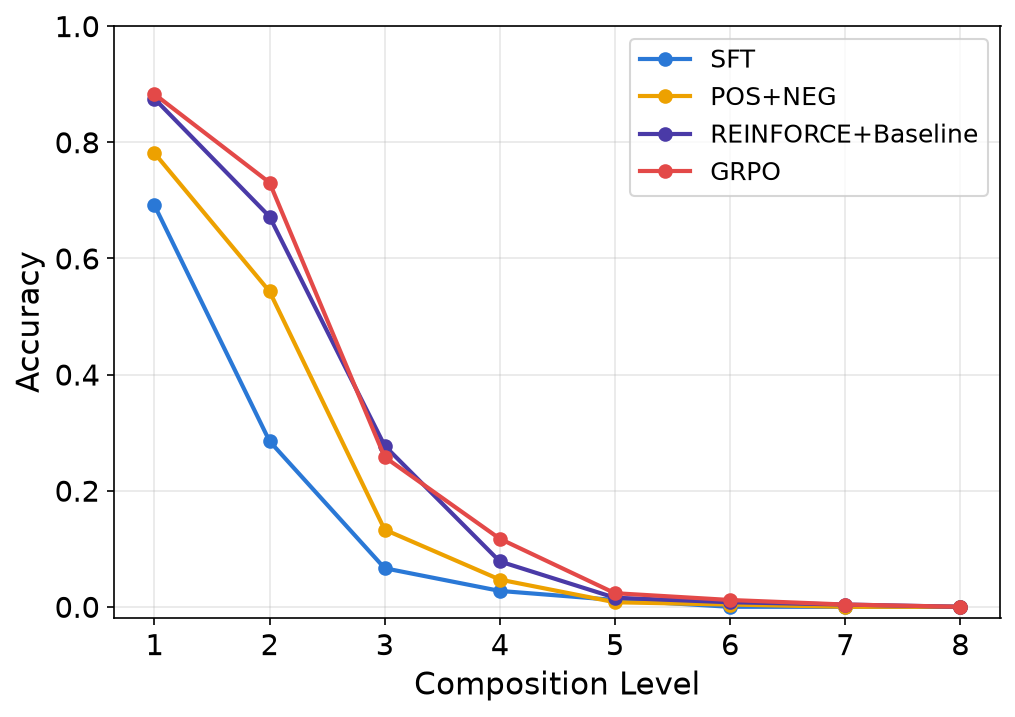
\includegraphics[width=0.8\textwidth]{imgs/loss_fn_on_policy.png}
\caption{Accuracy comparing different loss functions under On-policy setting on string function task}
\label{fig:generalization-zone-accuracy-string}
\end{figure}

\begin{figure}[h!]
\centering
\begin{subfigure}[b]{0.3\textwidth}
    \centering
    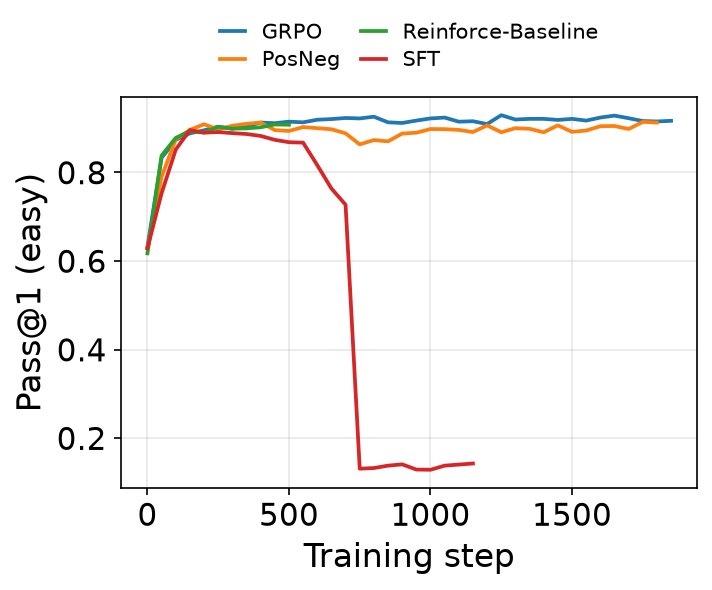
\includegraphics[width=\textwidth]{imgs/math_qwen3_pass1_easy.png}
    \caption{Accuracy on easy set}
    \label{fig:math_easy}
\end{subfigure}
\hfill
\begin{subfigure}[b]{0.3\textwidth}
    \centering
    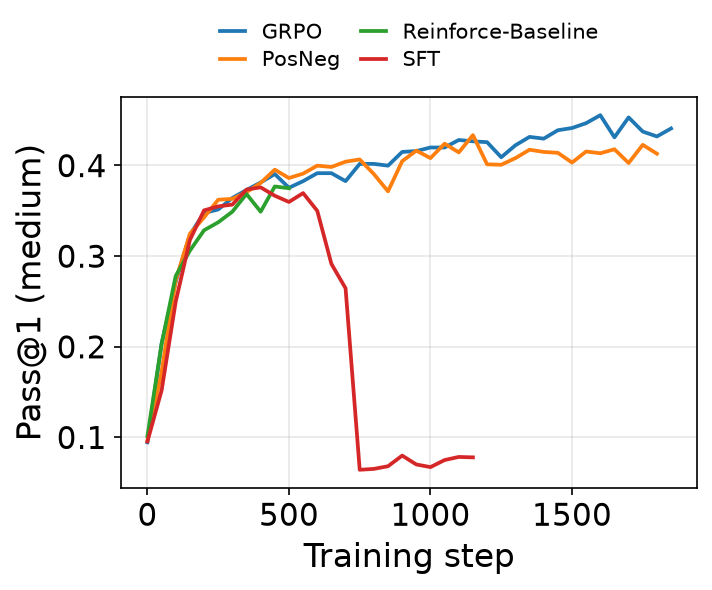
\includegraphics[width=\textwidth]{imgs/math_qwen3_pass1_medium.png}
    \caption{Accuracy on medium set}
    \label{fig:math_medium}
\end{subfigure}
\hfill
\begin{subfigure}[b]{0.3\textwidth}
    \centering
    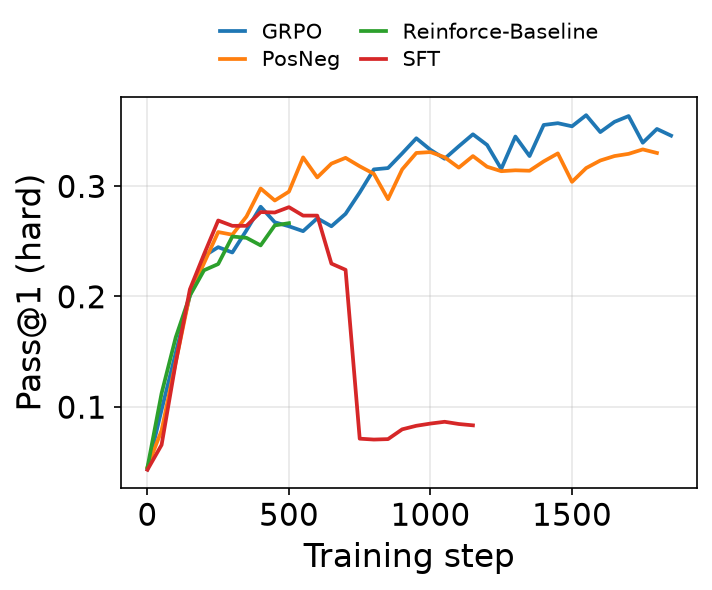
\includegraphics[width=\textwidth]{imgs/math_qwen3_pass1_hard.png}
    \caption{Accuracy on hard set}
    \label{fig:math_hard}
\end{subfigure}
\caption{Validation accuracy on math task \el{The text of these figures is way too small, they are pretty unreadable} \jk{Regenerated with panel-appropriate fonts (\texttt{scripts/analysis/plot\_math\_qwen3\_wandb\_metrics.py}, sized for 3-across at 0.3\textwidth); should be legible now.}}
\label{fig:generalization-zone-accuracy-math}
\end{figure}

\begin{figure}[h!]
\centering
\begin{subfigure}[b]{0.48\textwidth}
    \centering
    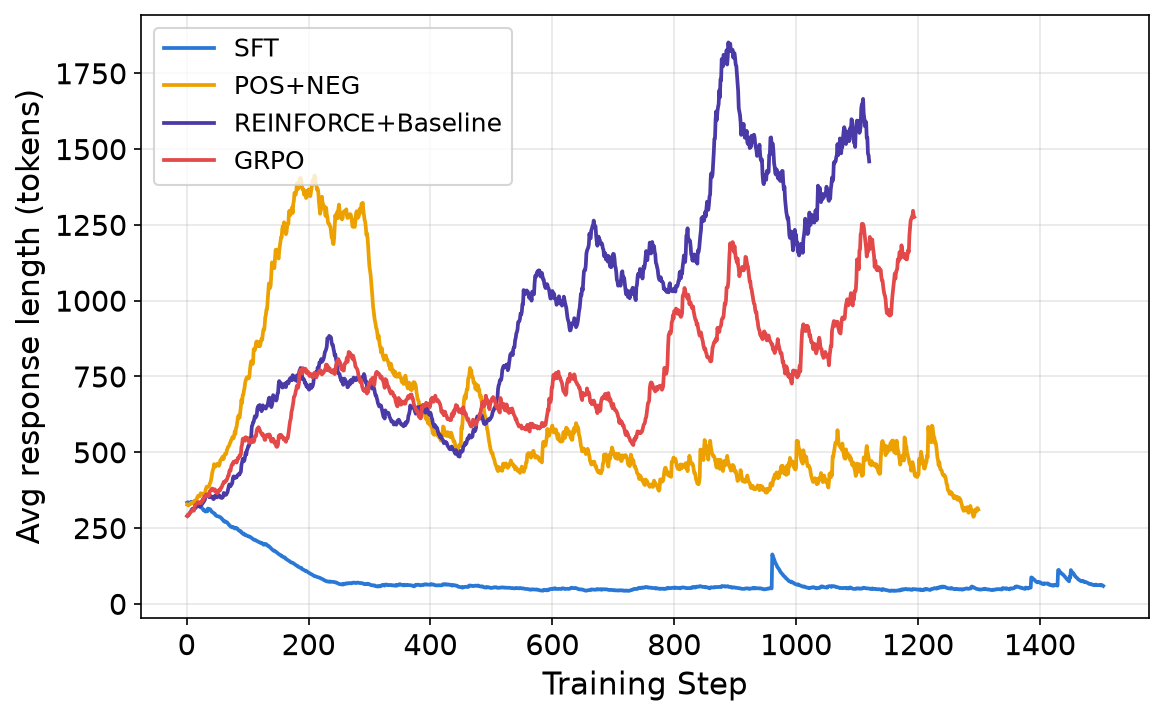
\includegraphics[width=\textwidth]{imgs/response_length.png}
    \caption{String task response length}
    \label{fig:response_length_a}
\end{subfigure}
\hfill
\begin{subfigure}[b]{0.48\textwidth}
    \centering
    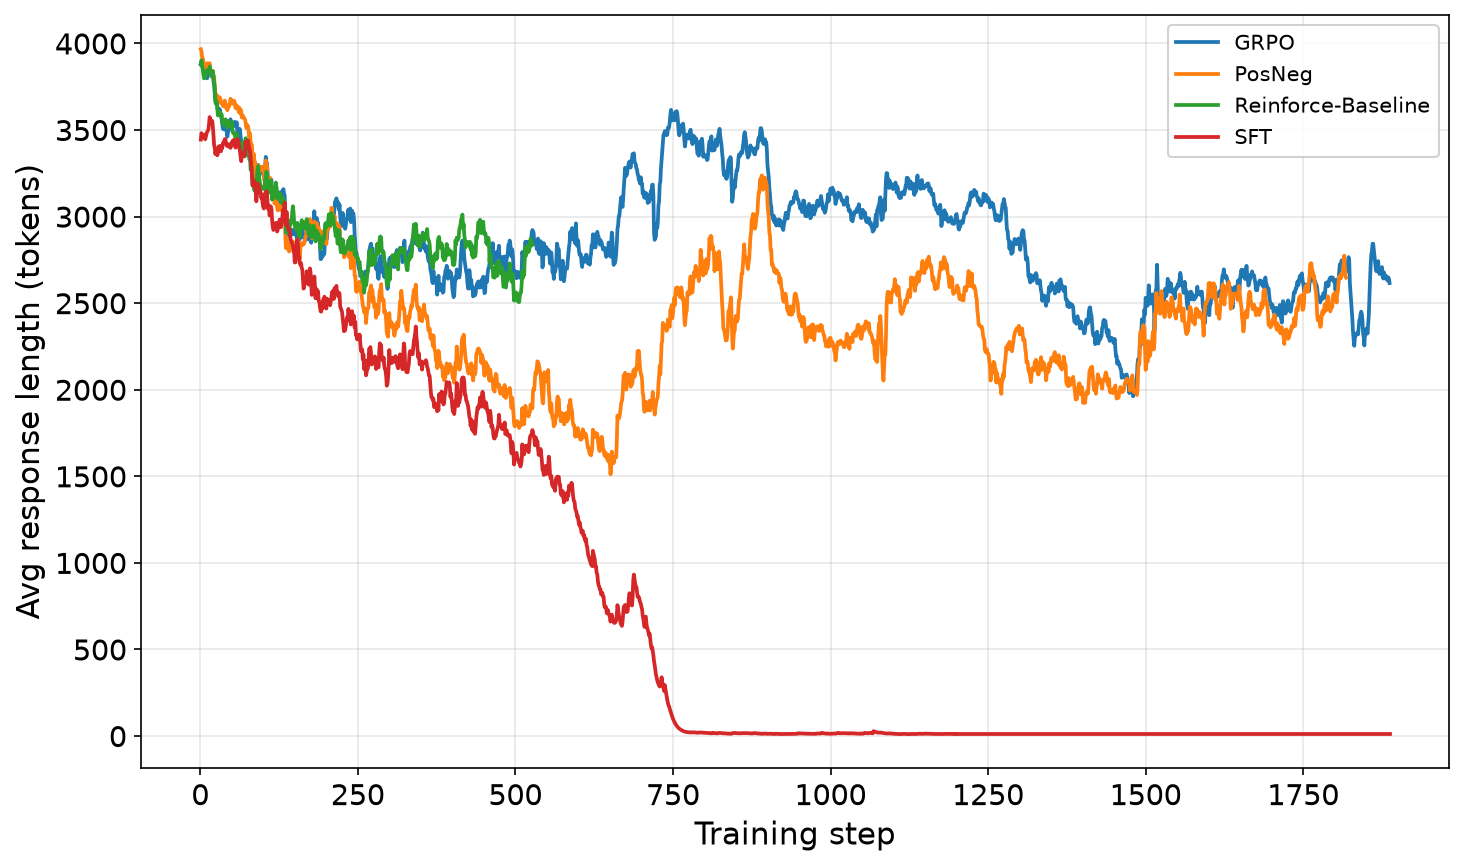
\includegraphics[width=\textwidth]{imgs/math_qwen3_response_length.png}
    \caption{Math task response length \el{The sft line seems cut off?} \jk{Confirmed real, not a rendering bug: the On-policy SFT run's wandb logging genuinely stops at step 1198, since the job was ended once response length had collapsed to $\sim$0 (Section \ref{sec:experiments} / \texttt{reports/math\_task\_response\_length\_dynamics.md} \S5), while GRPO/PosNeg continued to $\sim$1900. Extended flat to the other runs' range instead of leaving it truncated.}}
    \label{fig:response_length_b}
\end{subfigure}
\caption{Accuracy and Average response length over training steps under On-policy data setting on string function task}
\label{fig:response_length}
\end{figure}

\el{It actually seems both on and off policy methods don't generalize to level 5+ and the difference between on and off policy is kind of minor. I wonder if we can say something about this, also maybe we can do an avg. accuracy across levels (1-5) to kind of have one number to report rather than needing to look carefully at two figures}
\jk{Table \ref{tab:avg-acc-levels} gives that single number. All methods (on- and off-policy alike) are within noise of 0 by level 6, confirming the level 5+ observation. On the loss-function axis the ordering is clean and monotonic (SFT $<$ POS+NEG $<$ REINFORCE+Baseline $\approx$ GRPO); on the data axis, averaged over levels 1--5, On-policy-SFT (21.6\%) is statistically indistinguishable from Bootstrap-SFT (21.6\%) and only Teacher-SFT (25.3\%) pulls ahead, so "on-policy vs.\ off-policy" alone is a weak predictor for the SFT loss specifically --- the loss function axis matters far more than the data axis once you fix positive-only SFT.}

\begin{table}[h!]
\centering
\begin{tabular}{lc}
\toprule
\textbf{Method (on-policy data)} & \textbf{Avg. accuracy, Levels 1--5} \\
\midrule
SFT & 21.6\% \\
POS+NEG & 30.2\% \\
REINFORCE+Baseline & 38.4\% \\
GRPO & 40.2\% \\
\bottomrule
\end{tabular}
\caption{Single-number summary of Figure \ref{fig:generalization-zone-accuracy-string}: accuracy averaged over composition levels 1--5 (computed from \texttt{results/main.csv}).}
\label{tab:avg-acc-levels}
\end{table}

Finally, we observe the training behavior of different loss functions under the On-policy setting. For the string function task, Figure \ref{fig:generalization-zone-accuracy-string} shows that the gap between using SFT loss and GRPO loss is large. By adding negative samples (POS+NEG setting), we see that we can recover a significant chunk of the performance. However, there is still a performance gap, suggesting that naively adding negative gradients is not enough. Only after adding a baseline (REINFORCE+Baseline setting), we achieve very close to GRPO performance. This suggests that group-mean baseline is a key factor while standard-deviation normalization has relatively smaller impact. Similarly, Figure \ref{fig:generalization-zone-accuracy-math} illustrates the validation performance on easy, medium, and hard sets at various training steps. GRPO achieves best overall performance, but for this task, the gap between the 3 negative gradient methods are relatively small.

% Response length analysis
\subsection{Training Dynamics}

% \el{I think this should be a separate section?}

To analyze the training dynamics, we first look at response length. Figure \ref{fig:response_length} shows the average response length during training. Crucially, we see that SFT loss (only training on positive samples) contracts response length significantly. On the other hand, by training on negative samples as well, response length is maintained (for math task) and even increases during training (for string function task). 
We see that in GRPO and REINFORCE+Baseline settings, the response length increases steadily throughout training, achieving best performance around 1000 training steps. Interestingly, POS+NEG setting shows more instability in training as response length rapidly increases in the first stage, then gradually returns back to the Base model's levels. 
A possible explanation for this is that in the POS+NEG setting, the total magnitude of positive weights and negative weights are unbalanced. For example, if a group has much more positive samples than negative samples, the magnitude of positive gradient updates is much larger than that of negative gradient updates. By adding a baseline (REINFORCE+Baseline, GRPO settings), we balance the magnitude of gradient updates from positive and negative samples. As a result, POS+NEG setting is more sensitive to the difficulty of tasks while GRPO and REINFORCE+Baseline settings are more stable, eventually achieving greater performance.

Figure \ref{fig:entropy} plots eval-time entropy (averaged over depth-2 validation rollouts) throughout training. \jk{Pulled directly from wandb (\texttt{val/16-codeio-forward-incomplete-depth2/entropy/avg}); revising the claim below to match what the data actually shows.} Entropy for On-policy SFT collapses to effectively 0 by step $\sim$400 and stays there for the rest of training. POS+NEG, REINFORCE+Baseline, and GRPO instead hold a low but non-zero entropy band ($\sim$0.02--0.04) throughout, rather than increasing --- the key contrast is SFT's collapse-to-zero versus every negative-gradient method's stable non-zero floor, not a steady rise for GRPO specifically. As a result, negative-gradient methods provide more stable training, leading to a more successful model.

\begin{figure}[h!]
\centering
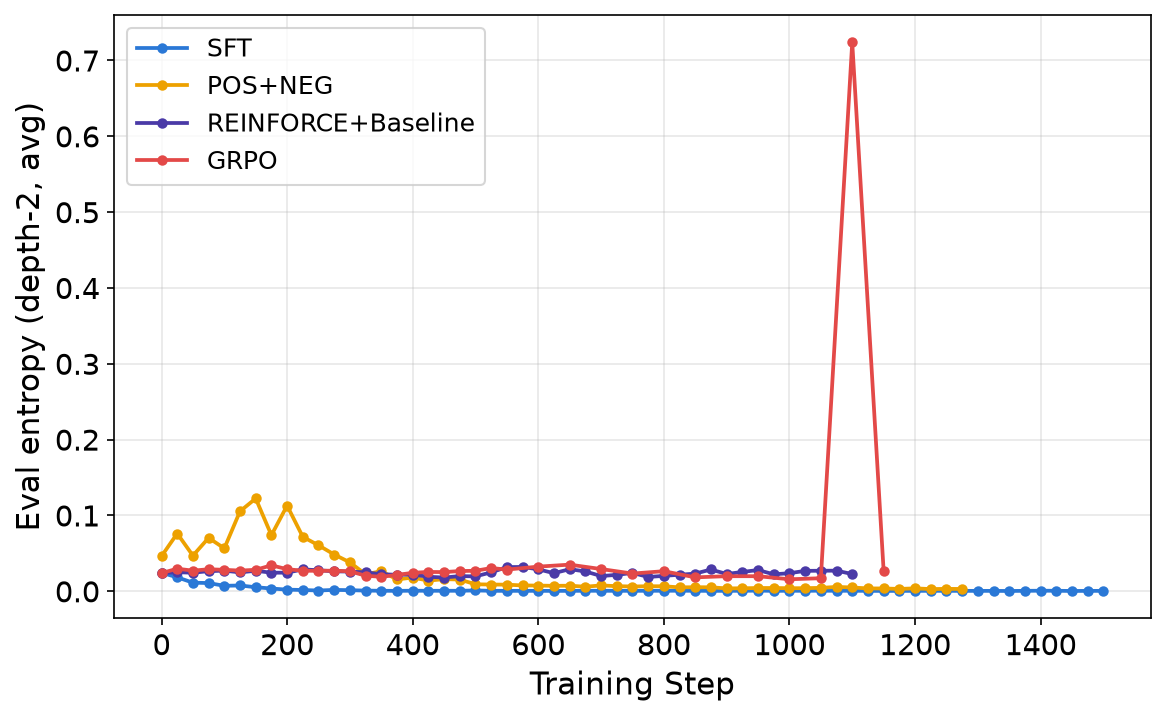
\includegraphics[width=0.6\textwidth]{imgs/entropy.png}
\caption{Eval entropy (depth-2 validation set, averaged) over training steps, on-policy setting.}
\label{fig:entropy}
\end{figure}

Figure \ref{fig:grad-norm} plots \texttt{actor/grad\_norm} over training for the same four on-policy runs. On-policy methods generally maintain a steady gradient norm (range 0.2--0.4) throughout training. However, in later stages of training, the On-policy SFT method shows increasingly frequent and large spikes in gradient norm (up to $5\times$ the stable band), revealing an instability in training that is absent for the three negative-gradient losses. This is consistent with the same run's entropy collapse in Figure \ref{fig:entropy}: as the policy's output distribution sharpens toward near-zero entropy, individual high-confidence-but-wrong updates produce disproportionately large gradients.

\begin{figure}[h!]
\centering
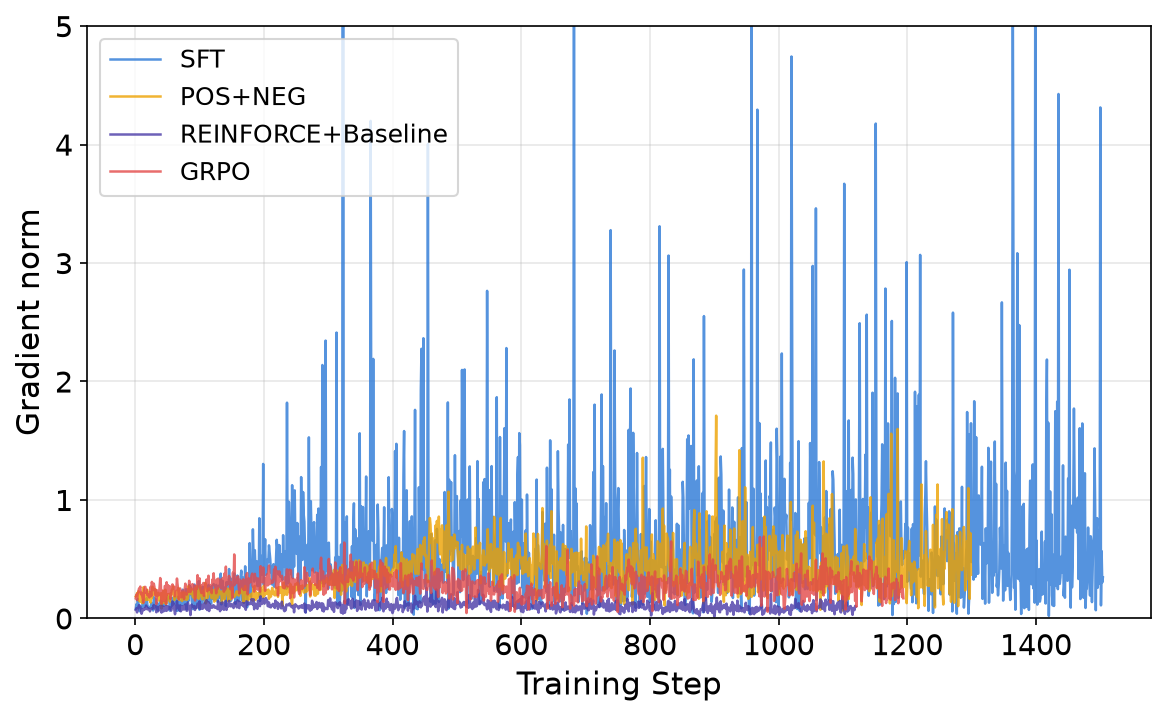
\includegraphics[width=0.6\textwidth]{imgs/grad_norm.png}
\caption{Gradient norm over training steps, on-policy setting (y-axis clipped at 5 for readability; see Figure \ref{fig:grad-norm-collapse} for the full off-policy comparison on a log scale).}
\label{fig:grad-norm}
\end{figure}


\section{Related Works}
\label{sec:related-works}
\textbf{Training Large Reasoning Models}

Post-training techniques for reasoning-capable LLMs have evolved rapidly, from early bootstrapping via self-generated traces \citep{zelikmanSTaRBootstrappingReasoning2022} and RLHF \citep{ouyangTrainingLanguageModels2022} to more recent systems demonstrating that zero-RL from a base model can produce strong reasoning, with supervised cold-starts further stabilizing training \citep{deepseek-aiDeepSeekR1IncentivizingReasoning2025}. 

A central debate concerns whether RL primarily \emph{sharpens} probability mass of existing solutions, improving pass@1 while reducing diversity \citep{yueDoesReinforcementLearning2025,wuInvisibleLeashWhy2026,zhaoEchoChamberRL2025}. The exploration view holds that RL can discover qualitatively new strategies \citep{zengSimpleRLZooInvestigatingTaming2025}, and methods such as entropy regularization \citep{cuiEntropyMechanismReinforcement2025}, representation-space novelty bonuses \citep{tuylsRepresentationBasedExplorationLanguage2025}, and experience replay strategies \citep{douImprovingRLExploration2025,zhangRLEPReinforcementLearning2025,zhanExGRPOLearningReason2025} have been proposed to preserve exploration throughout training.


\textbf{SFT versus Reinforcement Learning}

SFT and RL produce qualitatively different distributional changes: SFT improves in-distribution accuracy via memorization while RL generalizes out-of-distribution by exploiting latent model capabilities, and SFT can stabilize format for downstream RL \citep{chuSFTMemorizesRL2025}. At the trajectory level, RL compresses incorrect completions while SFT expands correct ones \citep{matsutaniRLSqueezesSFT2025}. Formally, SFT can be viewed as maximizing a lower bound on a sparse-reward RL objective \citep{qinSupervisedFineTuning2025}, and SFT, DPO-style objectives, and RL share a common policy-gradient structure differing primarily in data-generating policy, outcome weighting, and stabilization constraints \citep{lvUnifiedViewLarge2026}, with entropy serving as a useful training diagnostic when combining both signal types \citep{fuSRFTSingleStageMethod2025}. RL also mitigates catastrophic forgetting more effectively than SFT at matched performance, primarily due to on-policy data collection \citep{chenRetainingDoingRole2025,laiReinforcementFineTuningNaturally2026}, with SFT inducing a directional drift from prior capabilities that RL counteracts \citep{wuGeneralizationSFTReinforcement2025}. While prior work studies SFT and RL separately, this paper takes a finer-grained approach by analyzing their component-wise contributions.



\textbf{Extrapolation, Chaining, and Compositional Generalization}

Compositional generalization is the task of recombining known atomic operations in novel arrangements. This remains a significant challenge for LLMs, which often fail when individually mastered skills must be chained \citep{pressMeasuringNarrowingCompositionality2023,zhaoExploringCompositionalDeficiency2024,sunOMEGACanLLMs2025}, with data coverage requirements growing super-linearly with task diversity unless models exploit compositional structure \citep{abedsoltanTaskGeneralizationAutoRegressive2025}. Evidence that RL helps is growing: RL enables models to compose $f(g(x))$ from separately learned components where off-policy SFT fails \citep{yuanLLMsLearnNewSkills2025}, RL with compositional curricula yields genuine capability acquisition beyond sharpening \citep{motwaniH1BootstrappingLLMs2025}, composable chain-of-thought data facilitates systematic chaining \citep{yinLearningComposableChainsofThought2025}, and mid-training can bridge pre- and post-training distributions to establish the base-model competence that RL requires \citep{zhangInterplayPreTrainingMidTraining2025}.


\textbf{On-Policy Training}

A recurring theme is that the SFT–RL performance gap is largely attributable to the off-policy versus on-policy distinction rather than the loss form \citep{mingOneTokenRolloutGuiding2026}, and removing KL regularization and group-wise normalization from GRPO reduces it to on-policy SFT while still achieving competitive performance with shorter traces \citep{zhaoOnPolicySupervisedFineTuning2026}. However, on-policy SFT does not generally close the full gap to RL, suggesting that negative gradients and objective normalization provide additional independent signal.


\textbf{Role of Negative Gradients in Training}

Standard SFT provides only positive gradients, while RL implicitly applies negative updates by suppressing below-average completions, but the causal contribution of this signal has received limited direct study. Naive use of negative samples introduces failure modes: in DPO, the contrastive loss can reduce preferred-response likelihood \citep{pal_smaug_2024}, and in GRPO, Lazy Likelihood Displacement causes undifferentiated penalization to suppress correct response probability \citep{deng_effect_2025}. Yet both works find that targeted negative feedback is beneficial when applied carefully. Complementary evidence shows that negative trajectories with valid intermediate steps but incorrect final answers improve out-of-domain generalization and boost inference-time entropy \citep{tian_learning_2026}, with higher-quality negatives yielding greater gains \citep{di_not_2026}. This paper provides direct causal evidence for the negative gradient's contribution to compositional generalization, isolating it from the on-policy data effect and generalizing the use of negative samples in terms of sample weights.




\section{Conclusion}

We set out to answer a question that has become increasingly central to LLM post-training: \emph{what makes reinforcement learning effective for compositional reasoning, and which of its many ingredients are responsible?} Modern RL pipelines such as GRPO bundle on-policy rollouts, negative gradients, group-mean baselines, variance normalization, KL regularization, and curriculum schedules into a single training procedure, making it difficult to attribute observed gains to any specific mechanism. Prior work has illuminated individual components in isolation, but no controlled study has placed them in a common framework that allows for direct head-to-head comparison.

To address this, we proposed a unified two-axis decomposition of post-training methods. The \emph{data} axis ranges from teacher-distilled and bootstrapped off-policy data to fully on-policy rollouts, while the \emph{loss} axis ranges from positive-only SFT through positive-plus-negative gradients, REINFORCE with a group-mean baseline, and finally to the full GRPO objective. This grid places SFT, on-policy SFT, DPO, and GRPO as instances of a shared design space and exposes the components that distinguish them. We instantiated this framework on the string-function composition task, which provides a clean, controllable test of compositional generalization where the SFT-versus-RL gap is large and easily measurable.

Our experiments yield a clear hierarchy among RL components. On the data axis, on-policy data alone is insufficient: positive-only on-policy SFT contracts response length and entropy and underperforms teacher-distilled off-policy SFT at higher composition levels. On the loss axis, introducing negative gradients on top of on-policy training recovers a large fraction of the gap to GRPO, identifying the use of negative samples as the primary driver of compositional ability. Adding a group-mean baseline closes nearly all of the remaining gap, while the additional standard-deviation normalization in full GRPO contributes relatively little. Taken together, the bulk of GRPO's advantage on compositional generalization comes from the combination of on-policy rollouts and negative gradients with a stabilizing baseline, rather than from group-wise variance normalization or other objective-level details.

These findings carry two broader implications. First, they support a \emph{component-level} view of post-training: rather than treating RL as a monolithic improvement over SFT, practitioners can mix and match individual components (negative gradients, baselines, on-policy data) to obtain most of RL's benefits at lower implementation and compute cost. Second, they sharpen the ongoing debate over why RL works for reasoning. Our results are consistent with the view that negative gradients enable the model to suppress unproductive reasoning patterns rather than merely sharpen existing ones, and that on-policy data primarily serves to make this negative signal informative rather than to drive learning on its own.

This paper contributes a unified framework, a controlled set of ablations, and a concrete attribution of GRPO's advantage to the joint use of on-policy rollouts and baseline-stabilized negative gradients. We hope these results help shift post-training research toward principled, component-wise analysis, and ultimately toward more transparent and efficient training of reasoning-capable language models.



\section*{Limitations}
Several limitations remain. Our conclusions are established on a single controlled toy task and a single backbone model, and the binary, exactly verifiable reward of the string-function setting is simpler than rewards encountered in math and code benchmarks. Extending the decomposition to general reasoning tasks and to additional model families and sizes, as outlined in the Future Work chapter, is necessary to determine which parts of the component hierarchy are universal and which are task- or model-specific.
%%%%%%%%%%%%%%%%%%%%%%%%%%%%%%%%%%%%%%%%%%%%%%%%%%%%%%%%%%%%
\bibliographystyle{plainnat}
\bibliography{main}

\newpage
\appendix
\section{Training Details}


%%%%%%%%%%%%%%%%%%%%%%%%%%%%%%%%%%%%%%%%%%%%%%%%%%%%%%%%%%%%

\newpage
\input{checklist.tex}



\end{document}